\documentclass[a4paper, 12pt]{article}

\usepackage[utf8]{inputenc}
\usepackage[spanish]{babel}
\usepackage[margin=1.5in]{geometry}
\usepackage{graphicx}
\usepackage{float}
\usepackage{pdfpages}
\usepackage{listings}
\usepackage{listingsutf8}
\usepackage{xcolor}
\usepackage{scrextend}
\usepackage{array, multirow}
\usepackage{booktabs}
\usepackage{tabularx}

\definecolor{mGreen}{rgb}{0,0.6,0}
\definecolor{mGray}{rgb}{0.5,0.5,0.5}
\definecolor{mPurple}{rgb}{0.58,0,0.82}
\definecolor{backgroundColour}{rgb}{0.95,0.95,0.92}

\newcolumntype{C}[1]{>{\centering\arraybackslash}p{#1}}

\lstset{
language=C,
%backgroundcolor=\color{backgroundColour},   
commentstyle=\color{mGreen},
%keywordstyle=\color{magenta},
keywordstyle=\color{blue},
%numberstyle=\tiny\color{mGray},
stringstyle=\color{mPurple},
tabsize=4,
basicstyle=\fontsize{11}{13}\ttfamily\footnotesize,
showspaces=false,
showstringspaces=false,
captionpos=b,
breaklines=true
}

%\lstdefinestyle{CStyle}{
%    backgroundcolor=\color{backgroundColour},   
%    commentstyle=\color{mGreen},
%    keywordstyle=\color{magenta},
%    numberstyle=\tiny\color{mGray},
%    stringstyle=\color{mPurple},
%    basicstyle=\footnotesize,
%    breakatwhitespace=false,         
%    breaklines=true,                 
%    captionpos=b,                    
%    keepspaces=true,                 
%    numbers=left,                    
%    numbersep=5pt,                  
%    showspaces=false,                
%    showstringspaces=false,
%    showtabs=false,                  
%    tabsize=2,
%    language=C
%}

\title{		\textbf{Trabajo Práctico 3}\\
			\textbf{Data path y pipeline}
			}
			
\author{	Lucas Medrano, \textit{Padrón Nro. 99247}                     	\\
            \texttt{ lucasmedrano97@gmail.com }                           		\\
            Federico Álvarez, \textit{Padrón Nro. 99266}                 	\\
            \texttt{ fede.alvarez1997@gmail.com }                                 	\\[2.5ex]
            \normalsize{Grupo Nro. \quad - 2do. Cuatrimestre de 2018}      	\\
            \normalsize{66.20 Organización de Computadoras}               	\\
            \normalsize{Facultad de Ingeniería, Universidad de Buenos Aires}\\
       }
\date{}

\begin{document}
	\lstset{inputencoding=utf8/latin1} % Incorpora acentos en los listings
	\maketitle
	\thispagestyle{empty}
	\begin{abstract}
		El objetivo de este trabajo es implementar algunas instrucciones en dos configuraciones de una CPU en un emulador de MIPS32: CPU uniciclo, y CPU pipeline.
		Para implementar las instrucciones se deberá modificar tanto el set de instrucciones como el datapath de la CPU.  
	\end{abstract}
			
	\pagebreak
	\thispagestyle{empty}
	\tableofcontents
	\newpage
	
	\setcounter{page}{1}
	
	\section{Desarrollo}
	El trabajo se divide en dos partes:
	\begin{enumerate}
    \item Implementar las instrucciones en una CPU uniciclo.
    \item Implementar las instrucciones en una CPU pipeline.
	\end{enumerate}
	Las instrucciones que se implementaron son las siguientes:
	\begin{enumerate}
    \item andi Rs, Rt, Imm (And immediate). Esta instrucción de tipo I carga en Rs el resultado
de hacer un AND entre el contenido del registro Rt y el valor de 16 bits Imm.
    \item j Rs, Rt (Jump Rs+Rt). Esta instrucción de tipo I carga en el PC el resultado de sumar
los contenidos de los registros Rs y Rt.
	\item lw Rs, Rd*shamt(Rt). Esta instrucción de tipo R carga en el registro Rs la palabra de 32 bits
cuya dirección es Rt + Rd * shamt. Esta última sólo se implementara en la cpu uniciclo.
	\end{enumerate}
	
	\subsection{Implementación}
	\subsubsection{Programa}
	Para realizar el tp se usó el emulador DrMIPS, el cual permite visualizar el datapath que se usa, escribir programas, y seguir tanto el recorrido del programa y las señales en el datapath, como los valores de los registros.
	Modificando los archivos .cpu se modificaron ambos datapaths (unicycle y pipeline), y modificando los archivos .set se adecuaron ambos set de instrucciones para poder implementar las nuevas instrucciones.	
	
	\subsubsection{andi - CPU uniciclo}
	Para esta instrucción no hizo falta agregar ninguna estructura nueva al datapath. Generando un nuevo codigo de operacion (op) y seteando las señales de control de la Unidad de Control y de la ALU  se pudo obtener el resultado deseado.
	
	\subsubsection{andi - CPU pipeline}
	Al igual que en la versión uniciclo, para implementar esta instrucción no hizo falta más que generar un nuevo \texttt{opcode}, indicando las señales de control necesarias. En este caso se seteo \texttt{ALUOp} en el valor correspondiente a la operación \texttt{and}, y \texttt{ALUSrc} se seteó a 1 para indicar que en la segunda entrada de la ALU debe ingresarse el valor del campo \texttt{imm}. 
	No fue necesario modificar nada para el manejo de \textit{hazards} ya que con el soporte ya proporcionado bastaba.
	 
	\subsubsection{jregs - CPU uniciclo}
	Para poder implementar esta instrucción no bastaban las estructuras que incluía el datapath uniciclo.
	Se agregó un multiplexor que, mediante una entrada de control, decide si la siguiente direccion de PC es el resultado de la operación de la ALU o es la que indica MuxjUMP (PC+4/branch addres o jump address). Así, se puede setear que se sumen los registros indicados por parámetro, y que la siguiente direccion del PC sea dicha suma.
	Se decidió llamar "jregs" a esta instrucción debido a que ya había una instrucción j en el set de instrucciones usado.
	\subsubsection{j - CPU pipeline}
	Para implementar \texttt{jump} se agregó un multiplexor que toma la salida del multiplexor que maneja los branches y la salida de la ALU. Para controlarlo, se agregó una señal de control llamada \textit{Jump}, que se setea únicamente por esta operación, y debió ser pasada a través de las distintas etapas del pipeline, lo que requirió agregar un bit más a los registros ID/EX y EX/MEM.
	
	Para el manejo de hazards se agregó una compuerta \texttt{Or} que toma las señales de Branch y Jump y se las conecta a los registros de cada etapa del pipeline en la entrada \textit{Flush}, para agregar un ciclo de stall cuando se ejecuta un salto.
	\subsubsection{lw - CPU uniciclo}
	Para implementar esta instrucción se tomaron algunas decisiones:
	\begin{enumerate}
	\item No modificar el datapath: Ya que hay que hacer una multiplicación y luego obtener el resultado del registro "LO" mediante la instrucción mflo, se optó por dejar el datapath igual, e implementar la instrucción como una pseudo-instrucción.
	\item Implementarla como lw r1, r2, shamt, r3, debido a la sintaxis de MIPS.
	\end{enumerate}
	Se implementó la instrucción como una pseudo-instrucción: se multiplicó el valor de shamt por el de r2, se le sumó el de r3, se pidió el dato de memoria de dicha instrucción y se lo almacenó en r1.
	Una idea fue agregar un adder, para poder hacer el producto en el mismo ciclo de reloj. Sin embargo, primero se necesitaba mover el resultado del registro "LO" a algún registro, por lo que se optó lo indicado previamente.
	
	
	\subsection{Datapaths}
	Los datapath utilizados, y modificados, para el trabajo quedaron de la siguiente manera.
	
		\begin{figure}[h]
	  		\centering
			    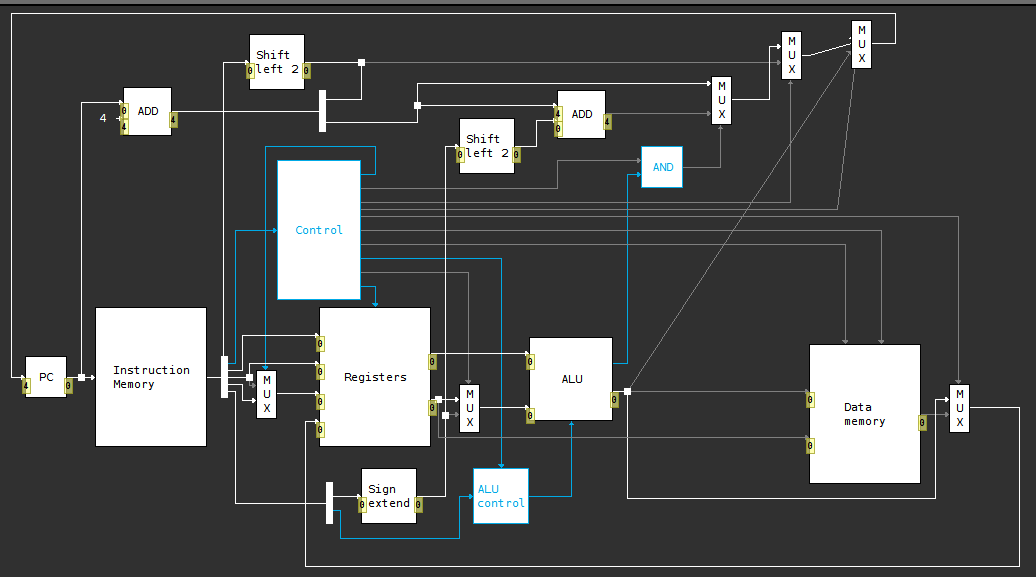
\includegraphics[width=\textwidth]{files/cpuunicycle.png}
		 	 \caption{Datapath de la CPU-Unicycle.}
	  		\label{fig}
		\end{figure}
	
		\begin{figure}[!h]
	  		\centering
			    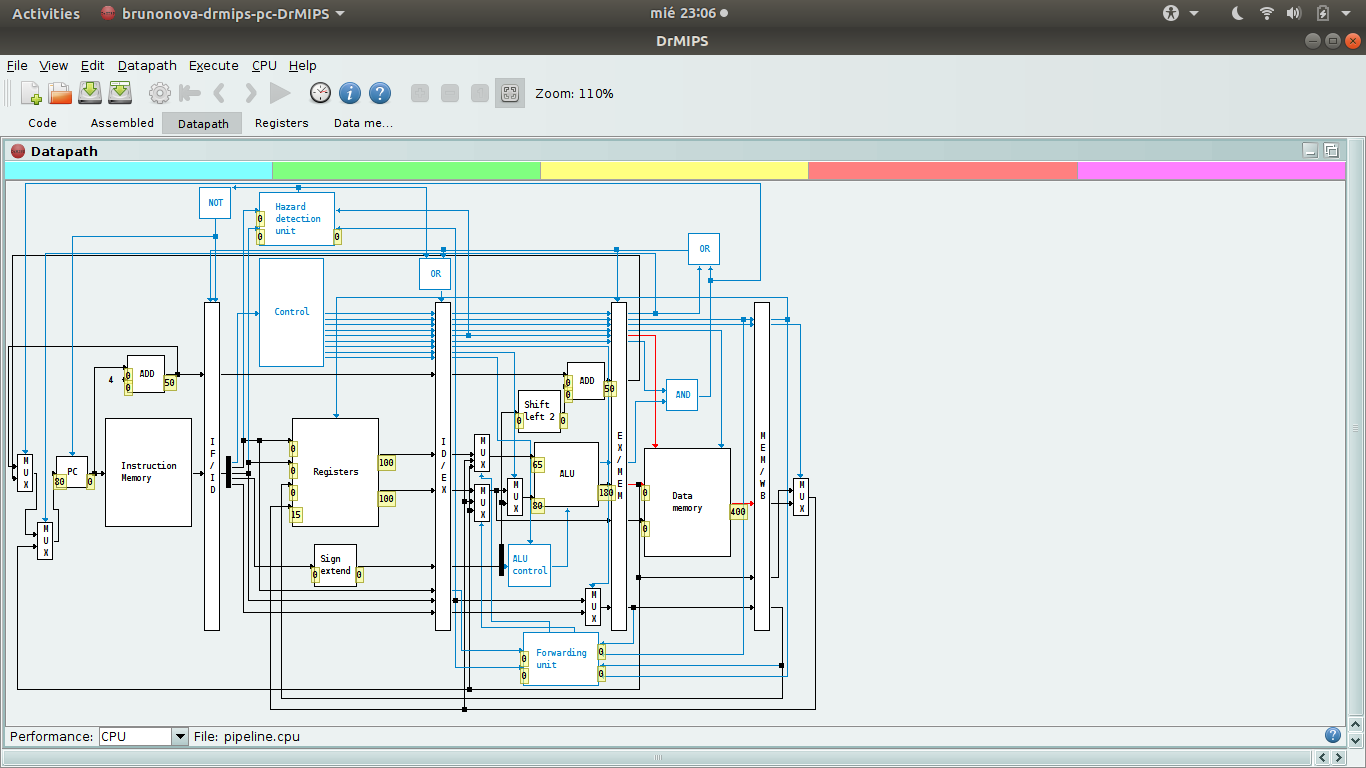
\includegraphics[width=\textwidth]{files/cpupipelined.png}
		 	 \caption{Datapath de la CPU-Pipelined.}
	  		\label{fig}
		\end{figure}	
	
	\subsection{Pruebas}
	Para cada instrucción implementada se agregan una, o más, pruebas para asegurarse que el comportamiento sea el esperado. Se adjuntan dichas pruebas a los archivos del trabajo.
	Para probar la instrucción andi, tanto en uniciclo como en pipeline, se setearon valores en los registros, se corrió la instrucción andi entre ellos, y se chequeó que los registros quedaran como se esparaba. 
	Similarmente para lw en la cpu uniciclo, se guardó un dato en memoria y luego se setearon valores en registros tales que la combinación que pide el lw diera la dirección de memoria en donde se habia guardado el dato, y se comparó que el dato cargado en el registro sea el que habíamos cargado en memoria.
	Para la instrucción jregs en la cpu uniciclo se setearon dos registros y luego se corrió la instrucción y se chequeó que el PC quede como se esperaba. Además, se añadió una instrucción que modificara algun registro luego del salto para ver si se tomaba, o no, y asi verificar si habia, o no, hazards.
	
	\section{Conclusiones}
	Se logró implementar las instrucciones pedidas.
	El trabajo nos ayudó a entender varios conceptos. Modificar el datapath, las estructuras y cableados permite entender mucho mejor el funcionamiento del procesador en general y de cada estructura en particular. Modificar los set de instrucciones ayuda a ver mucho mejor cómo influye el datapath utilizado a la hora de generar instrucciones. Aprendimos que el datapath define el set de instrucciones que se podrá utilizar, pero un mismo set de instrucciones puede ser implementado de varias maneras distintas (en este caso con un CPU uniciclo y uno Pipeline). Además, se logró conceptualizar la diferencia entre el CPU uniciclo y el CPU pipeline.
	EL programa DrMips fue de gran ayuda para poder visualizar no solo el datapath, los set de instrucciones, los registros en todo momento, sino también el camino que seguía cada instrucción en el datapath al ser ejecutada.

	
	\newpage
	\section{Apéndice}
	\subsection{Enunciado}

	\begin{figure}[H]
		\centering
		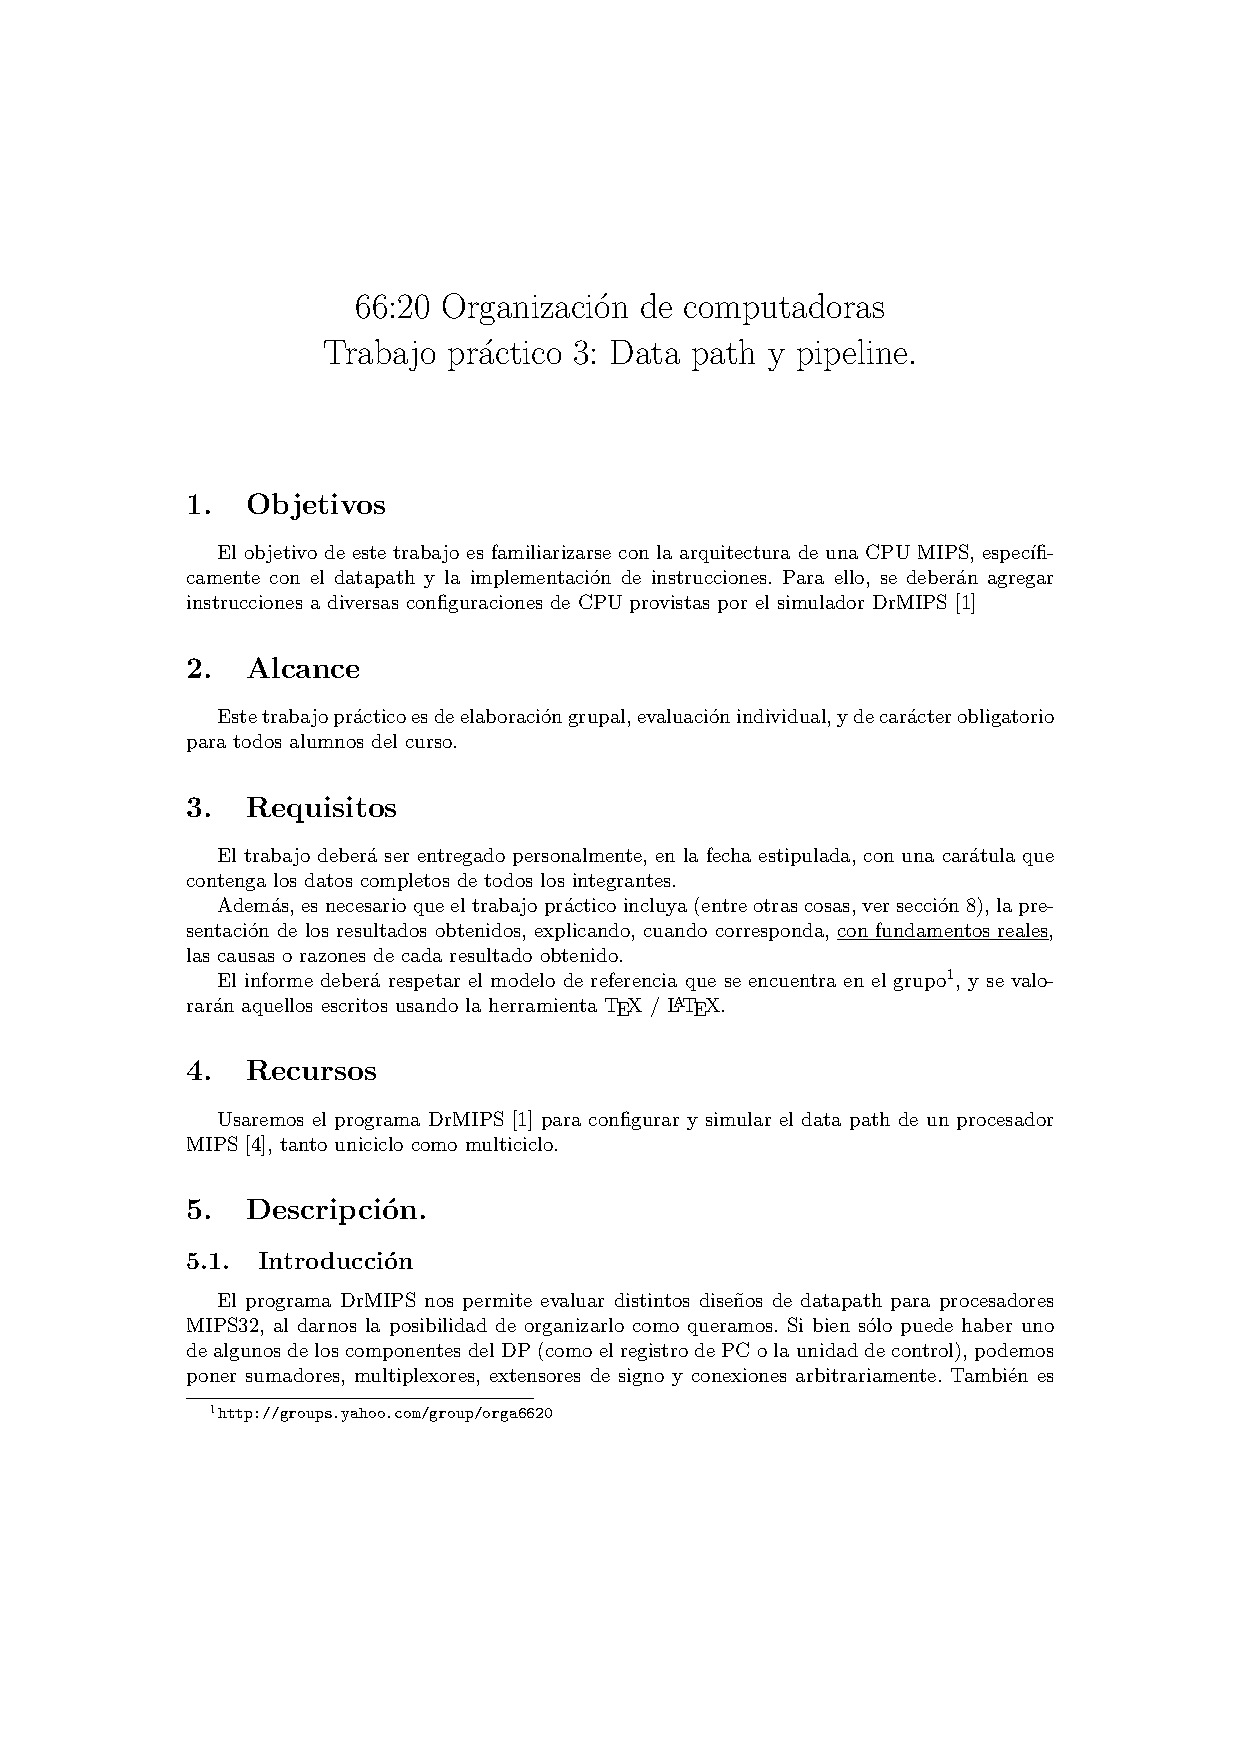
\includegraphics[scale=1, page = 1, clip, trim=1.2in 36mm 20mm 1.5in]{files/tp3-c2-2018.pdf}
	\end{figure}
	
	\newpage
	\begin{figure}[H]
		\centering
		\includegraphics[scale=1, page = 2, clip, trim=1.2in 2in 20mm 1.2in]{files/tp3-c2-2018.pdf}
	\end{figure}
	
	\newpage
	\begin{figure}[H]
		\centering
		\includegraphics[scale=1, page = 3, clip, trim=1.2in 2in 20mm 1.2in]{files/tp3-c2-2018.pdf}
	\end{figure}
	
	\newpage
	\begin{figure}[H]
		\centering
		\includegraphics[scale=1, page = 4, clip, trim=1.2in 2in 20mm 1.2in]{files/tp3-c2-2018.pdf}
	\end{figure}
	
\end{document}
